\section{Ziel}
In diesem Versuch soll die Ablenkung eines Elektronenstrahls durch eine elektrisches Feld untersucht werden.
Genauer zu bstimmen ist dabei von welchen Parametern die Ablenkung abhängt und die aus der theorie bestimmten Gleichungen sollen überprüft werden.
\section{Theorie}
\label{sec:Theorie}
Um Elektronenstrahlen zu untersuchen müssen experimentelle Aufbauten in einem Hochvakuum aufgebaut werden, damit die Elektronen nicht mit der Luft wechselwirken.
In diesem Experiment wird dazu eine sogenannte Kathodenstrahlröhre verwendet, die mit einem Vakuum von bis zu $10^{-6}$ mbar Restdruck arbeitet.
Die Kathodenstrahlröhre besteht dabei im wesentlichen aus drei Bauteilen, einer "Elektronenkanone", einem Ablenksystem und einem Nachweissystem.
\begin{figure}[H]
    \centering
    \includegraphics[width=0.4\textwidth]{bilder/Querschnitt.png}
    \caption{Bild Querschnitt}
    \label{fig:Querschnitt}
\end{figure}
Der Elektronenstrahl wird dabei in der "Elektronenkanone" erzeugt. 
Die "Kanone" besteht aus einem Zylinder aus einem Kathodenmaterial, welches eine geringe Austrittsarbeit hat,
und einem darinliegenden elektrich vom Zylinder isolierten, Heizdraht der Rot glüht.
Um diese Glühkathode herum befindet sich mit etwas Zwischenraum ein sogenannter Wehnelt zylinder, welcher negativ geladen ist und einen kleines rundes Loch in Richtung des Schirms besitzt.
Mit der negativen Ladung des Wehnelt zylinders werden die Elektronen nicht nur in die entsprechende Richtung gelenkt, sondern es lässt sich auch die Intensität des Elektronenstrahls steuern.
Unmittelbar nach dem Wehnelt Zylinder befindet sich eine positiv geladene Beschleunigungselektrode, welche die Elektronen auf die Geschwindigkeit $v_{\text{Z}}$ (nach Gl. \ref{eqn:Beschleunigung}) beschleunigt.
\begin{align}
    \frac{ m_0 v_{\text{Z}}^2}{2}= e_0 U_{\text{B}} \nonumber \\
    v_{\text{Z}} = \sqrt{\frac{2 e_0 U_{\text{B}}}{m_0}} \label{eqn:Beschleunigung}
\end{align}
Nach der Beschleunigungselektrode durchläuft der Elektronenstrahl noch einen Aufbau einer elektronischen Linse, die den erzeugten Strahl fokussiert.
Die Brechkraft der Linse kann dabei über die Spannung $U_{\text{C}}$ (Abb. \ref{fig:Querschnitt}, rechte Seite) verändert werden.
Nach diesem Aufbau der "Elektronenkanone" befinden sich 2 Plattenpaare die der Ablenkung des Strahls in X und Y Richtung dienen.
Die Normalen der beiden Plattenpaare stehen dabei senkrecht zueinander, so dass jedes Plattenpaar nur Einfluss auf eine Komponente der Elektronengeschwindigkeit hat.
Die Ablenkung hängt dabei sowohl von der Geschwindigkeit der Elektronen, als auch von der Angelegten Kondensatorspannung ab, näheres dazu in \ref{sec:Ablenkung}.
Der nun abgelenkte Elektronenstrahl fällt nun auf das Nachweissystem, welches aus einem speziell beschichteten Leuchtschirm innerhalb der Kathodenröhre besteht.
Wenn nun Elektronen die Aktivatorzellen auf dem Schirm anregen geben diese Lichtquanten ab und der Beobachter kann den Punkt bestimmen an dem die Elektronen auftreffen.
Der Lichtschirm ist dabei elektrisch mit der Beschleunigungselektrode verbungden, damit der Schirm sich nicht negativ auflädt.
\subsection{Ablenkung}
\label{sec:Ablenkung}
\begin{figure}[H]
    \centering
    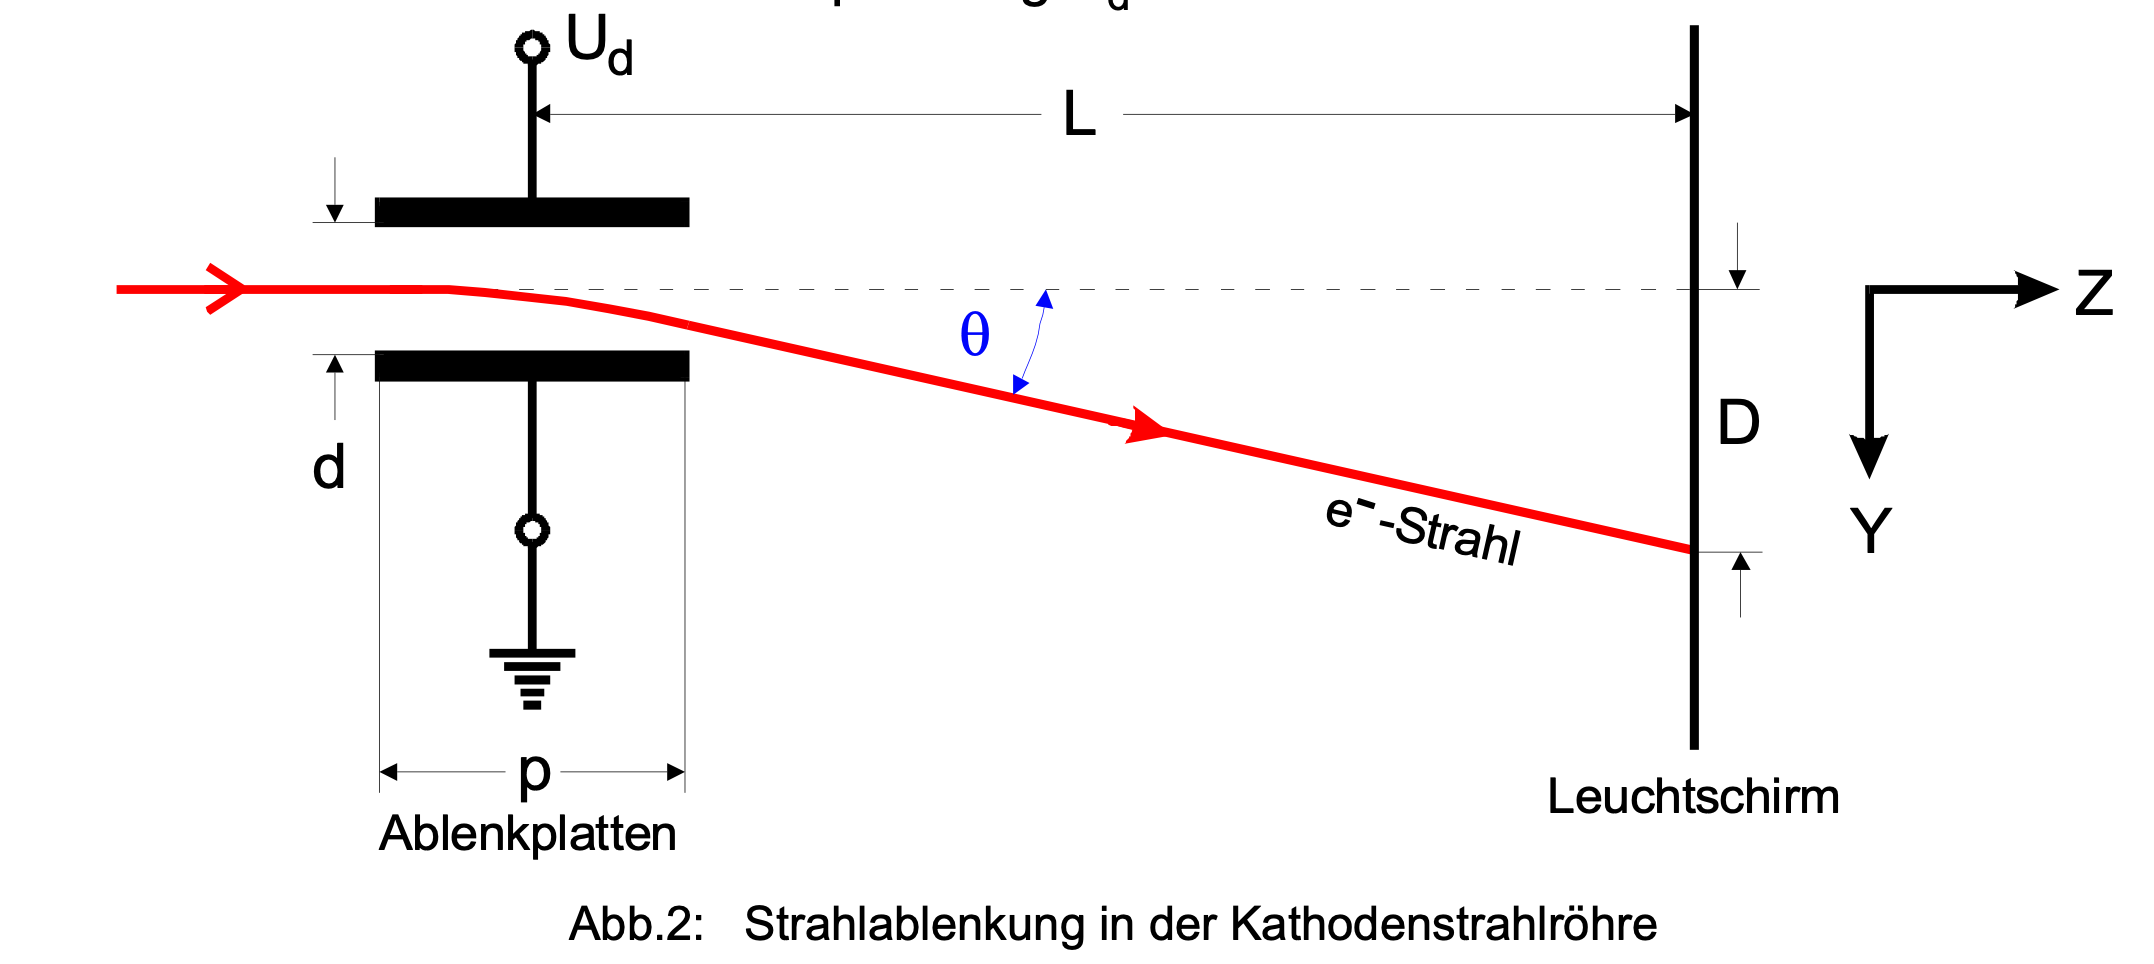
\includegraphics[width=0.4\textwidth]{bilder/Strahlablenkung.png}
    \caption{Bild Strahlablenkung}
    \label{fig:Strahlablenkung}
\end{figure}
Wenn der Plattenabstand $d$ klein gegenüber der Plattenbreite $p$ ist kann für das induzierte elektriche Feld angenommen werden:
\begin{equation*}
    E = \frac{U_{\text{d}}}{d}
\end{equation*}
Damit ergibt sich für die Kraft auf die Elektronen im Feld
\begin{equation}
    |\bar{F}| = |e_0\bar{E}| = e_0 \frac{U_{\text{d}}}{d} \label{eqn:Kraft}
\end{equation}
Zusammen mit \ref{eqn:Kraft} ergibt sich somit für ein Elektron welches in der Zeit $\Delta t$ durch den Plattenkondensator fliegt die Geschwindigkeit
\begin{equation}
    v_{\text{y}} = a_{\text{y}} \Delta t = \frac{F}{m_0}\Delta t = \frac{e_0 U_{\text{d}}}{m_0 d} \Delta t
\end{equation}
Die Zeit in der das Elektron die Platten durchfliegt lässt sich mit der Geschwindigkeit der Elektronen vor dem Kondensator bestimmen $\Delta t = \frac{p}{v_{\text{z}}}$ und damit ergibt sich
\begin{equation}
    v_{\text{y}}  = \frac{e_0 U_{\text{d}} p}{m_0 d v_{\text{z}}} 
\end{equation}
Der Ablenkwinkel $\theta$ über den im Anschluss die Verschiebung $D$ des Auftrittpunktes auf dem Schirm berechnet wird ergibt sich Ablenksystem als 
\begin{equation}
    \theta ≈ \frac{v_y}{v_z} = \frac{e_0 U_{\text{d}} p}{m_0 d v_{\text{z}}^2}
\end{equation}
Und damit
\begin{equation}
    D = \theta L = \frac{v_y}{v_z} = \frac{e_0 U_{\text{d}} p}{m_0 d v_{\text{z}}^2} L
\end{equation}
Die Geschwindigkeit $v_{\text{z}}$ lässt sich über die Spannung an der Beschleunigungselektrode bestimmen (\ref{eqn:Beschleunigung})und wir erhalten
\begin{equation}
    D = \frac{p}{2d}L\frac{U_d}{U_B}
\end{equation}
Es ist nun leicht zu erkennen, dass die Ablenkung proportional zur Spannung des Kondensators ist, und somit lässt sich der Aufbau auch nutzen um Spannungen zu messen.
Allerdings müssen beim Betrieb der Kathodenstrahlröhre auch Kompromisse eingegangen werden.... 
\subsection{Kathodenstrahl Oszillograph}
Die Kathodenstrahlröhre kann sehr leicht umfunktioniert werden um den zeitlichen Verlauf einer Wechselspannung zu untersuchen.
Dazu wird an den Plattenkondensator für die horizontale X-Richtung eine Sägezahnspannung angeschlossen und an den Kondensator in Y-Richtung wird die untersuchte Wechselspannung angeschlossen.
Wenn nun beide Frequenzen in einem bestimmten Verhältnis stehen, lässt sich auf dem Lichtschirm der zeitliche Verlauf der Wechselspannung betrachten.
\begin{equation}
    n\cdot \nu_{\text{Sä}} = m\cdot \nu_{\text{We}}
\end{equation}
Dieses Verhältnis mit $n = 1,2,3,...$ und $m = 1,2,3,...$ wird Synchronisationsbedingung genannt.